\documentclass[12pt,a4paper]{article}
\usepackage[french]{babel}
\usepackage[latin1]{inputenc}
\usepackage[T1]{fontenc}
\usepackage{vmargin}
\usepackage{pdfpages}
\setmarginsrb{2.5cm}{1.5cm}{2.5cm}{2cm}{0cm}{0cm}{0cm}{0cm}

\begin{document}
\pagestyle{empty}
{\sffamily
\noindent{Universit\'{e} de Lille \hfill Facult\'{e} de Pharmacie de Lille \\ Ann\'{e}e Universitaire 2022/2023}

\vspace{25mm}
\begin{center}
\textbf{THESE \\
POUR LE DIPLOME D'ETAT \\
DE DOCTEUR EN PHARMACIE}
\end{center}
\vspace{13mm}
\noindent{\textbf{\hspace*{13mm}Soutenue publiquement le xx/yy/2023 \\
\hspace*{13mm}Par M. RIHANI Emir Ka\"{i}s}}
\vspace{26mm}
\begin{center}
\rule{65mm}{0.8pt} \\
\vspace{6mm}
\textbf{APPLICATION DE MODELES D'INTELLIGENCE ARTIFICIELLE \\~\\ A LA CLASSIFICATION DES MACROMYCETES} \\
\vspace{2mm}
\rule{65mm}{0.8pt}
\end{center}
\vspace{45mm}
\noindent{\textbf{\underline{\smash{Membres du jury}} :} \\
~\\
\textbf{Pr\'{e}sident :} Nom, Prenom, titre et lieu de fonction \\
~\\
\textbf{Directeur, conseiller de th\`{e}se :} Nom, Prenom, titre et lieu de fonction \\
~\\
\textbf{Assesseur(s) :} Nom, Prenom, titre et lieu de fonction}
}
\newpage
~
\newpage
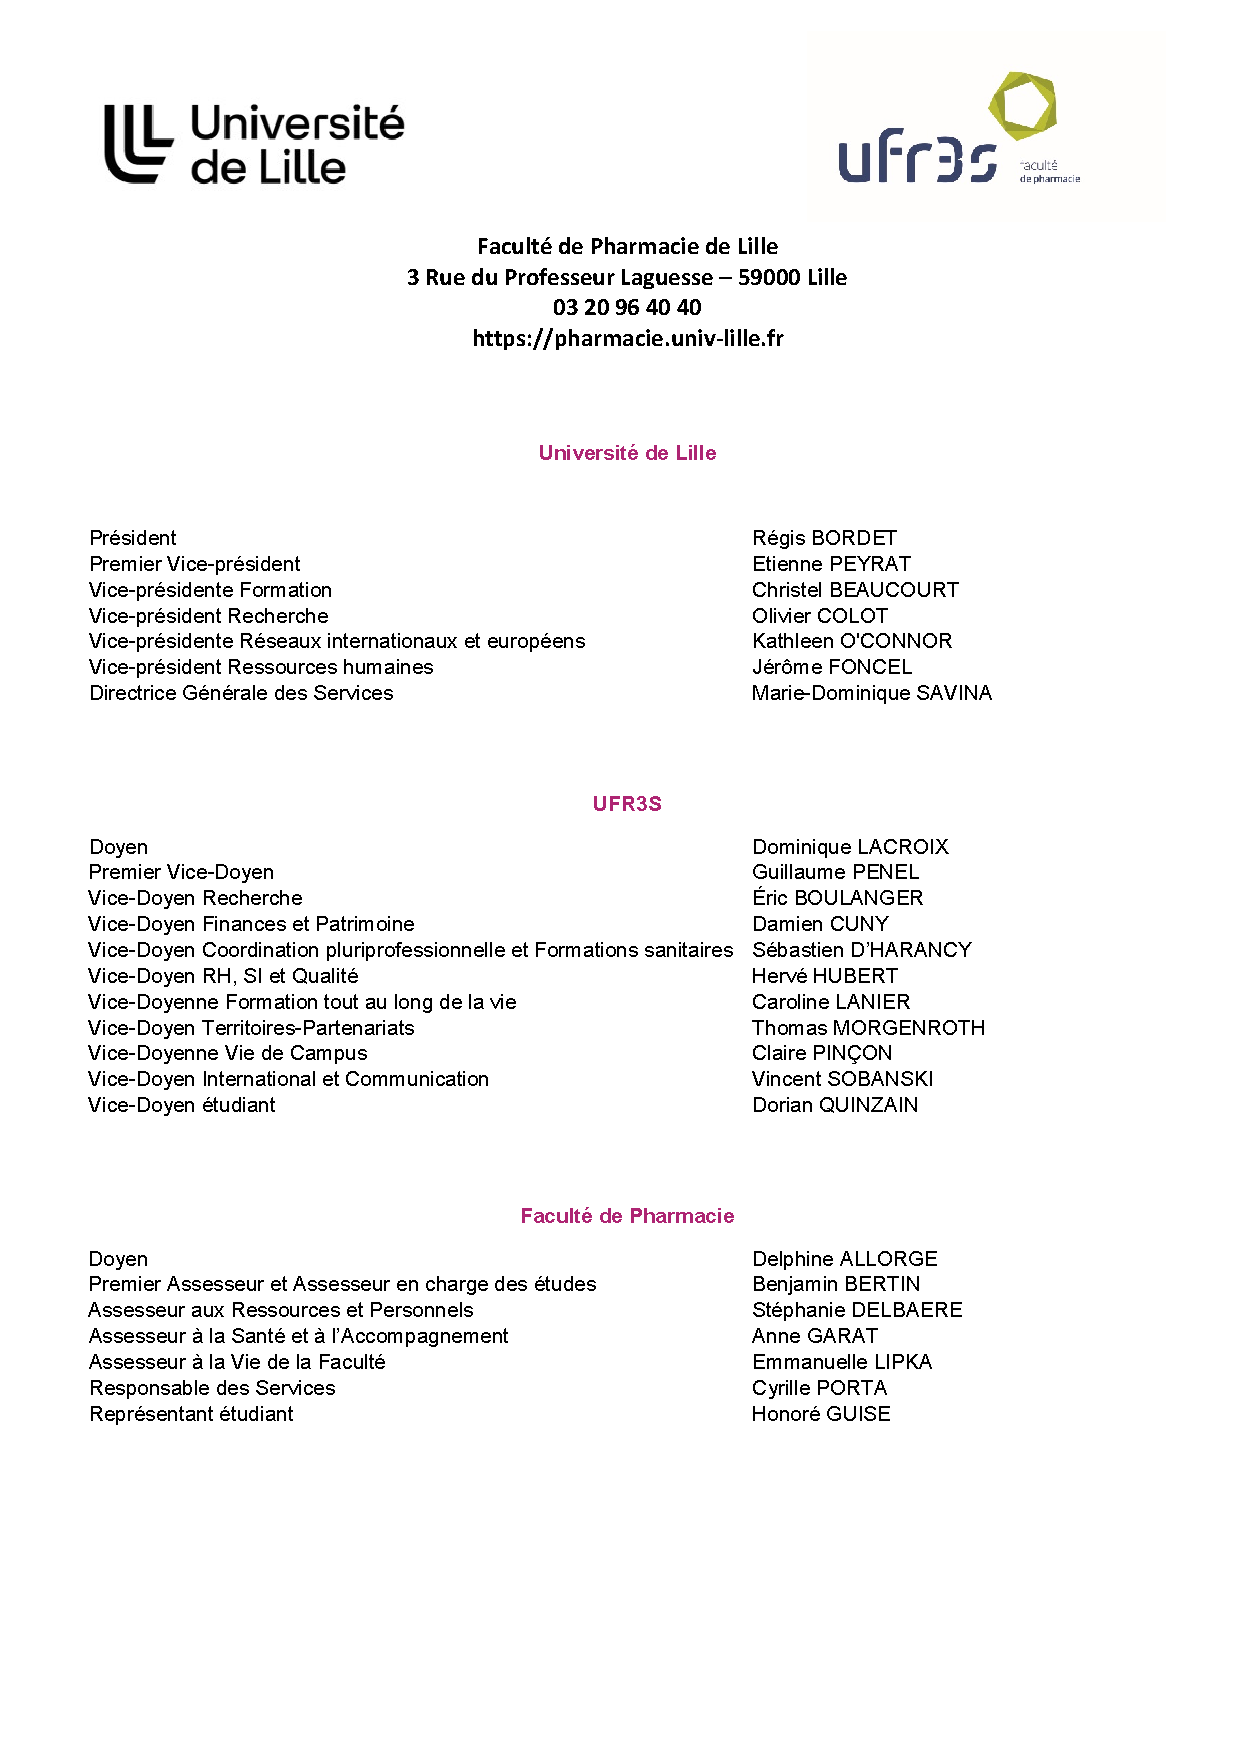
\includepdf[pages={-}]{liste_enseignants_2022.pdf}
\end{document}


